\chapter{Preliminares}\label{chapter: VRP}

En este trabajo se presenta el proceso de evaluación automática de las soluciones vecinas, que se obtienen en los algoritmos de búsqueda local, para cualquier VRP.

Este capítulo presenta los conceptos básicos de los problemas de enrutamiento de vehículos y los algoritmos de búsqueda local. Además, se definen los criterios de vecindad que se utilizan en el sistema y la estructura de datos que se utiliza para evaluar soluciones parciales de manera automática.

En la sección \ref{1-VRPintro} se presentan las características principales de los VRP. En la sección \ref{2-LocalSearch} se describen los algoritmos de búsqueda local. En la sección \ref{3-Criterias} se explican los criterios de vecindad que se utilizan en el sistema. En la sección \ref{3-EvalGraph} se describe el grafo de evaluación que se utiliza para evaluar las soluciones vecinas en cada VRP.

%\newpage

\section{Problema de Enrutamiento de Vehículos}\label{1-VRPintro}
Desde 1959, cuando George Dantzig y John Ramser introducen la primera definición de un VRP\cite{Dantzing}, se han desarrollado variantes asociadas a las demandas de los clientes del problema. Estas demandas pueden ser el tiempo de espera, la entrega y recogida de paquetes o la capacidad de los vehículos. 

Todos los VRP presentan uno o múltiples depósitos iniciales, de donde parten los vehículos para satisfacer las demandas de cada cliente. El recorrido termina en los depósitos.

A continuación, en \ref{fig:vrp-variants} se presentan esquemas de diferentes variantes de VRP. En la primera variante (CVRP) cada vehículo presenta una capacidad \cite{Alemany}. La segunda variante (VRPWT) muestra clientes con ventanas de tiempo \cite{Kolen}. En la tercera variante (MDVRP) se aprecia más de un depósito para la flota de vehículos \cite{Bayir, Alemany}. 


\begin{figure}
	\centering
	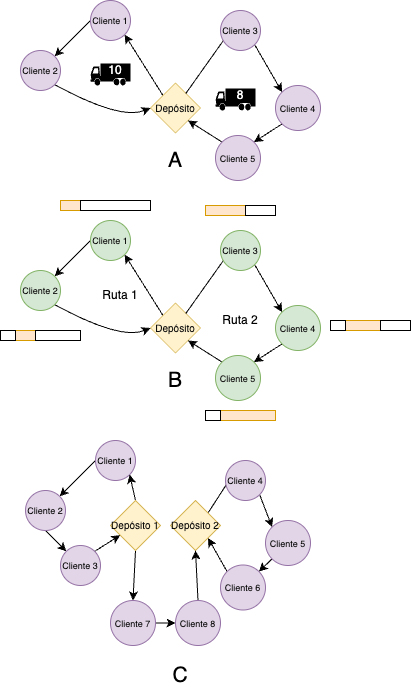
\includegraphics[width=0.7\linewidth]{Graphics/VRP}
	\caption{Variantes del VRP. A: CVRP. B: VRPTW. C: MDVRP.}
	\label{fig:vrp-variants}
\end{figure}

Como se puede notar, sería muy dificil encontrar un algortimo general que resuelva cualquier VRP, dado que estos problemas presentan restricciones diferentes y, por lo tanto, estrategias diferentes para solucionarlos. Estas estrategias son heurísticas o metaheurísticas que se adaptan a las características específicas de un tipo específico de VRP. En la siguiente sección se presenta la búsqueda local, en la que se basan un grupo de estas metaheurísticas.

%Soluciones con la búsqueda local

\section{Algoritmos de Búsqueda Local}\label{2-LocalSearch}

En los algoritmos de búsqueda local se parte de una solución inicial $S_{0}$, que se modifica de varias maneras para obtener un conjunto $NS_{0}$ llamado conjunto de soluciones vecinas de $S_{0}$, o vecindad de $S_{0}$\cite{JJ}. A las reglas que se aplican para modificar una solución y obtener las soluciones vecinas se les conoce con el nombre de estructura de entorno o criterio de vecindad\cite{JJ}. Del conjunto de soluciones $NS_{0}$ se extrae una nueva solución a modificar. Esto se realiza hasta cumplir con algún criterio de parada.

Existen diferentes algoritmos que se basan en la búsqueda local. Por ejemplo, \textit{Simulated Annealing}\cite{Liu}, \textit{Tabu Search}\cite{Taillard1997}, \textit{Variable Neighborhood Search}\cite{Camila}. Estos algoritmos difieren en los criterios utilizados para obtener las soluciones vecinas. La siguiente sección trata sobre esos criterios de vecindad.

%Criterios de vecindad
\section{Criterios de vecindad}\label{3-Criterias}

Los criterios de vecindad son reglas para transformar una solución de un problema determinado y obtener nuevas soluciones. Para el caso de VRP, estos criterios pueden ser \textit{``cambiar un cliente de posición''}, \textit{''intercambiar dos clientes''}, o \textit{''cambiar el vehículo de una ruta''}.

Estos criterios se pueden describir como una secuencia de operaciones elementales. Algunas de estas pueden ser:

\begin{enumerate}
	\item Seleccionar una ruta \texttt{r}. 
	\item seleccionar un cliente \texttt{c} de una posición \texttt{p} de una ruta \texttt{r}.
	\item insertar un cliente \texttt{c} en una posición \texttt{p} de una ruta \texttt{r}.
\end{enumerate}

Por ejemplo, el criterio \textit{cambiar un cliente de posición} está compuesto por las operaciones \textit{extraer cliente de una posición dada} e \textit{insertar al cliente en otra posición},
mientras que el criterio \textit{cambiar el vehículo de una ruta} puede componerse por las operaciones \textit{ extraer vehículo de ruta} y \textit{ asignar a una ruta dada un determinado vehículo disponible}.

Los criterios de vecindad utilizados en un algoritmo de búsqueda local dependen de la variante de VRP que se esté resolviendo \cite{Daniela}. Por ejemplo, en un problema donde la flota de vehículos es homogénea pero existen varios depósitos, la operación \textit{cambiar vehículo} no tiene sentido pero \textit{cambiar depósito} sí puede aplicarse.

Para evaluar cada una de las soluciones vecinas del VRP y aplicar los criterios de vecindad, se utiliza una estructura de datos llamada grafo de evaluación que se define en la siguiente sección. Este grafo se usa para evaluar de manera automática la solución del problema, es decir, sin que sea necesario escribir el código de la evaluación.

% Grafo de Evaluación
\section{Grafo de Evaluación}\label{3-EvalGraph}

A partir de la solución inicial del VRP se crea un grafo que se utilizará para evaluar las soluciones vecinas obtenidas por los criterios de vecindad en cada problema del VRP.

En \cite{JJ} se define formalmente la estructura del grafo de evaluación.

\begin{defn}
	Entidad del problema: Cada uno de los elementos que componen la solución de una determinada variante de un VRP.
\end{defn}
  
  Por ejemplo, en un problema con flota heterogénea las entidades del problema serían los clientes, los vehículos y el depósito central. En este trabajo se presentan como \textit{variables iniciales}.
  
  \begin{defn}
	  Información del problema: Dato que forma parte de la entrada del problema.
  \end{defn}
  
  Un ejemplo de información en el CVRP es la demanda de cada cliente y también la distancia entre cada par de clientes. Para el HFVRP, la capacidad
  de cada vehículo es también una información del problema.
  
  \begin{defn}
	Variable: Se refiere a toda variable que se use durante la evaluación de una solución y contenga un valor numérico que no sea información del problema ni entidad del problema.
  \end{defn}
  Ejemplos de variables serían \textit{distancia-total, demanda-de-ruta, }etc. En este trabajo se presentan como variables intermedias.


  \begin{defn}
	  Operación: Función que se aplica durante la evaluación de una solución.
  \end{defn}
  
  Durante la evaluación de una determinada solución es común aplicar operaciones entre las variables como \textit{incrementar distancia total, aumentar o disminuir la carga de un vehículo, penalizar exceso de carga,
  }etc.
  
  \begin{defn} \label{def:op-node}
	  Nodo operacional: Nodo que representa una operación.
  \end{defn}
  
  Un nodo operacional es la representación en el grafo de evaluación de una operación. Toda operación recibe una entrada y
  provoca que se transforme  una determinada salida. Por ejemplo, cuando se aplica la operación \textit{incrementa la distancia total en la distancia entre los clientes 1 y 2}
  se incrementa el valor contenido en la variable \textit{distancia-total} (salida) en dependencia de la distancia entre los clientes 1 y 2 (entradas).
  
 En este trabajo, los nodos operacionales son parte de las variables intermedias, y se les asocia la operación. También se le asocia dos métodos, el método de evaluación, que se utiliza para evaluar las demandas de las variables, y el método de desevaluación, que vuelve atrás la evaluación realizada; es decir hace la operación inversa de la evaluación.

  En la definición \ref{def:op-node} se establece la representación de una operación, por tanto se hace necesario definir la representación de las entradas y las salidas de dichas
  operaciones.
  
  \begin{defn}
	  Nodo de entrada/salida: Nodo que representa la entrada o la salida de alguna operación.
  \end{defn}
\subsection*{Construcción del grafo de evaluación}
Para construir este grafo, en primer lugar, se realiza un proceso de inicialización, donde se construyen únicamente los nodos principales de dicho grafo, que son los correspondientes a cada cliente y depósito. A continuación se muestra un ejemplo del grafo inicializado.

En el ejemplo se presentan 4 clientes (1,2,3,4) y dos rutas (A,B). Un vehículo comienza en un depósito y recorre a los clientes 1, 2 y 3 que se encuentran en A y regresa al depósito, otro vehículo visita al cliente 4 que pertenece a la ruta B:
\begin{displaymath}
A = [1,2,3]          B = [4]
\end{displaymath}
En la figura \ref{fig:vrp-initialGraph} se muestra cómo se inicializa el grafo.

\begin{figure}[htb]
	\centering
	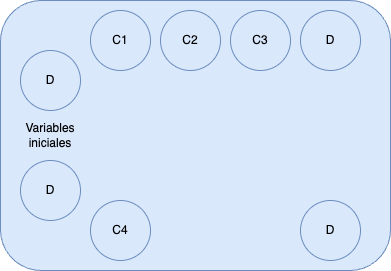
\includegraphics[width=0.7\linewidth]{Graphics/Init}
	\caption{Grafo inicializado.}
	\label{fig:vrp-initialGraph}
\end{figure}

Un grafo inicializado no contiene ninguna arista debido a que en un grafo de evaluación las aristas indican las entradas y las salidas de las operaciones que se realizan en la evaluación de la solución\cite{JJ}.

Luego de inicializado el grafo se desarrollan los nodos intermedios a partir del código de evaluación de la solución inicial. En la figura se presenta el código que evalúa una solución del VRP. La operación \texttt{d(x,y)} representa la distancia entre \texttt{x} e \texttt{y}.

\begin{lstlisting}
evaluate(S):
  new_var total_distance = 0
  for each route r in S:         
      new_var route_demand = 0
      new_var prev_client = depot(r)
      for each client c in r:
          increase total_distance with d(prev_client, c)
          increase route_demand with demand of client c
          prev_client = c
      increase total_distance with d(c, depot) 
      increase total_distance with penalize(demand_route, vehicle_capacity)
   return total_distance        
\end{lstlisting}

En ese proceso de evaluación se realizan operaciones para obtener el costo de la solución. Estos costos pueden ser la distancia recorrida, la demanda de la ruta, la penalización de la ruta, etc. Para guardar el resultado de estas operaciones se crean nuevos nodos, que llamaremos nodos intermedios.

A continuación se muestra el grafo de evaluación de la primera solución del VRP.

En la figura \ref{fig:vrp-Graph-process1} se muestra la creación de una variable intermedia asociada al cliente 1 para guardar el costo de la ruta del depósito al cliente 1. Además, se crea un nodo para guardar la penalización de la ruta y un nodo para guardar la suma total de la ruta 1.

\begin{figure}[htb]
	\centering
	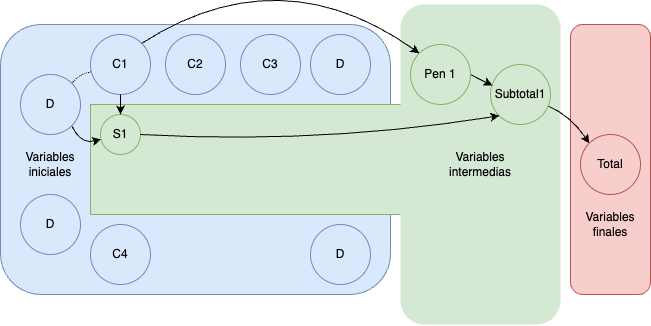
\includegraphics[width=0.7\linewidth]{Graphics/Graph-process}
	\caption{ Proceso del grafo de evaluación comenzando con el cliente 1.}
	\label{fig:vrp-Graph-process1}
\end{figure}

En la figura \ref{fig:vrp-Graph-process2} se muestra que la evaluación de la ruta 1 está calculada.

\begin{figure}[htb]
	\centering
	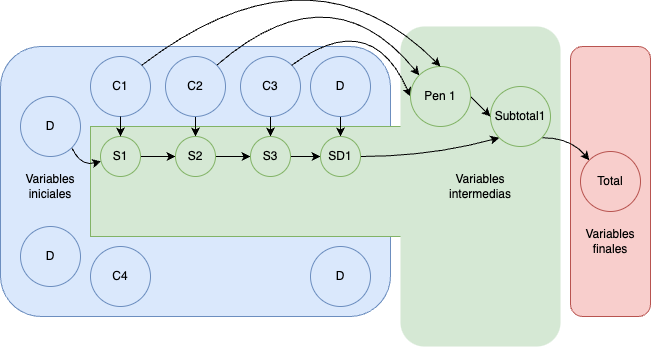
\includegraphics[width=0.7\linewidth]{Graphics/Graph-process2}
	\caption{Proceso del grafo de evaluación a terminar la ruta A.}
	\label{fig:vrp-Graph-process2}
\end{figure}

Por último, en la figura \ref{fig:vrp-Graph-process3} se presenta el grafo de evaluación para esta solución.

\begin{figure}[htb]
	\centering
	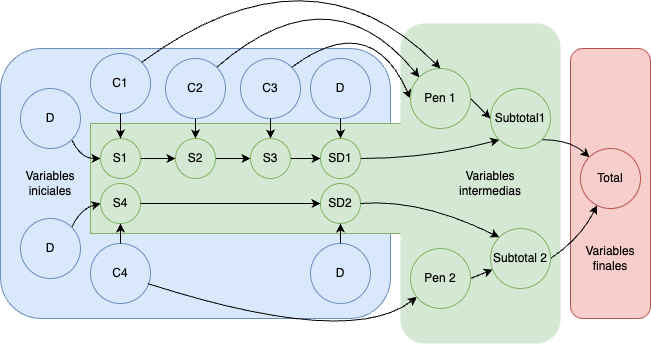
\includegraphics[width=0.7\linewidth]{Graphics/Graph-process3}
	\caption{Proceso del grafo de evaluación terminado.}
	\label{fig:vrp-Graph-process3}
\end{figure}

Se puede comprobar que el grafo ha guardado cada cálculo parcial de la evaluación de la solución en las variables intermedias creadas, de tal manera que, al aplicar un criterio de vecindad a la solución puede evaluarse sin necesidad de hacer el proceso de evaluación completo nuevamente. Si a la solución anterior se aplicara, por ejemplo, la operación eliminar cliente C3 como se muestra en la figura  \ref{fig:vrp-deleteClient} entonces no se modifica el valor del cálculo que se realizó antes de visitar este cliente o el valor calculado de otra ruta. 

La soluciones, que se obtienen cuando se aplica un criterio de vecidad a la solución anterior, pueden evaluarse de manera automática a partir de la solución previa, sin necesidad de escribir un nuevo código de evaluación. En el ejemplo \ref{fig:vrp-deleteClient} se pasa de la suma parcial del cliente 2 a la suma parcial del depósito.

\begin{figure}[htb]
	\centering
	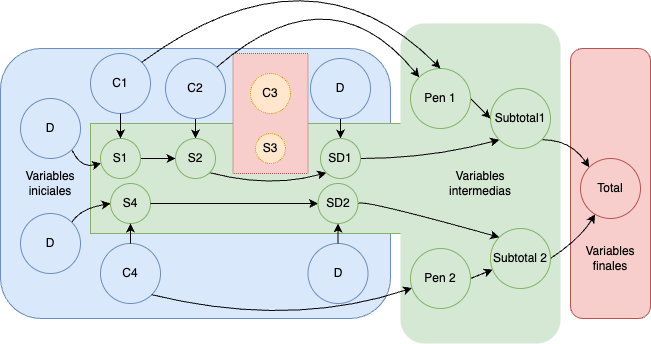
\includegraphics[width=0.7\linewidth]{Graphics/DeleteClient}
	\caption{Grafo de evaluación transformado al eliminar el cliente 3.}
	\label{fig:vrp-deleteClient}
\end{figure}

Otro ejemplo sería eliminar este cliente C3 en la ruta A e insertarlo en la ruta B como se presenta en la figura \ref{fig:vrp-changeClient}. En este caso, en la ruta A se evalúa sólo a partir de la suma parcial 2 como en el ejemplo anterior, ya que no se modifica el valor calculado previamente. Además, debe evaluarse la ruta B a partir del cliente insertado porque el valor calculado de la ruta hasta el cliente anterior no se modificó.

\begin{figure}[htb]
	\centering
	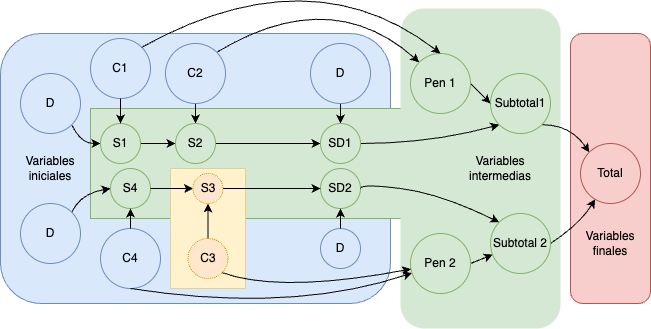
\includegraphics[width=0.7\linewidth]{Graphics/ChangeClient}
	\caption{Grafo de evaluación transformado al cambiar el cliente 3 de la ruta A a la ruta B.}
	\label{fig:vrp-changeClient}
\end{figure}

Los nodos intermedios hacen función de variables acumuladoras, porque guardan el costo de cumplir la demanda de cada cliente y las aristas describen el siguiente nodo a evaluar que depende del valor de nodo anterior.

El proceso de calcular a partir de un nodo o evaluar la ruta desde el depósito hasta el nodo final, depende de una cinta computacional que se conecta a este grafo de evaluación. La idea de esta cinta surge de la Diferenciación Automática que se explica en el siguiente capítulo.
% Chapter 2 Cinta de la Diferenciación automática

% Chapter 3 Mezcla y código en Lisp

% Chapter 4 Resultados

% Conclusiones, recomendaciones y bibliografía




























